\section{Motivation}
\label{sec:motivation}

We motivate carbon-aware FaaS scheduling with a joint characterization
of the two data sources that drive our design: a representative FaaS
workload, and the grid carbon-intensity signal that determines the
carbon footprint of executing that workload.

\subsection{Joint Characterisation}

Figure~\ref{fig:motivation} overlays a 48-hour grid carbon-intensity
trace for Germany --- a synthetic trace whose annual mean is
calibrated to the ENTSO-E 2020 figure later validated against real
LWA data in \S\ref{sec:evaluation:realcarbon} --- with the per-minute
invocation rate of a representative \code{webhook\_handler} function
drawn from a workload generator calibrated to the
\citet{shahrad2020serverless} Azure characterization. Shaded bands
mark the lowest-quartile (green) and highest-quartile (red) carbon
windows over the 48-hour horizon. Three observations emerge.

\begin{figure*}[t]
\centering
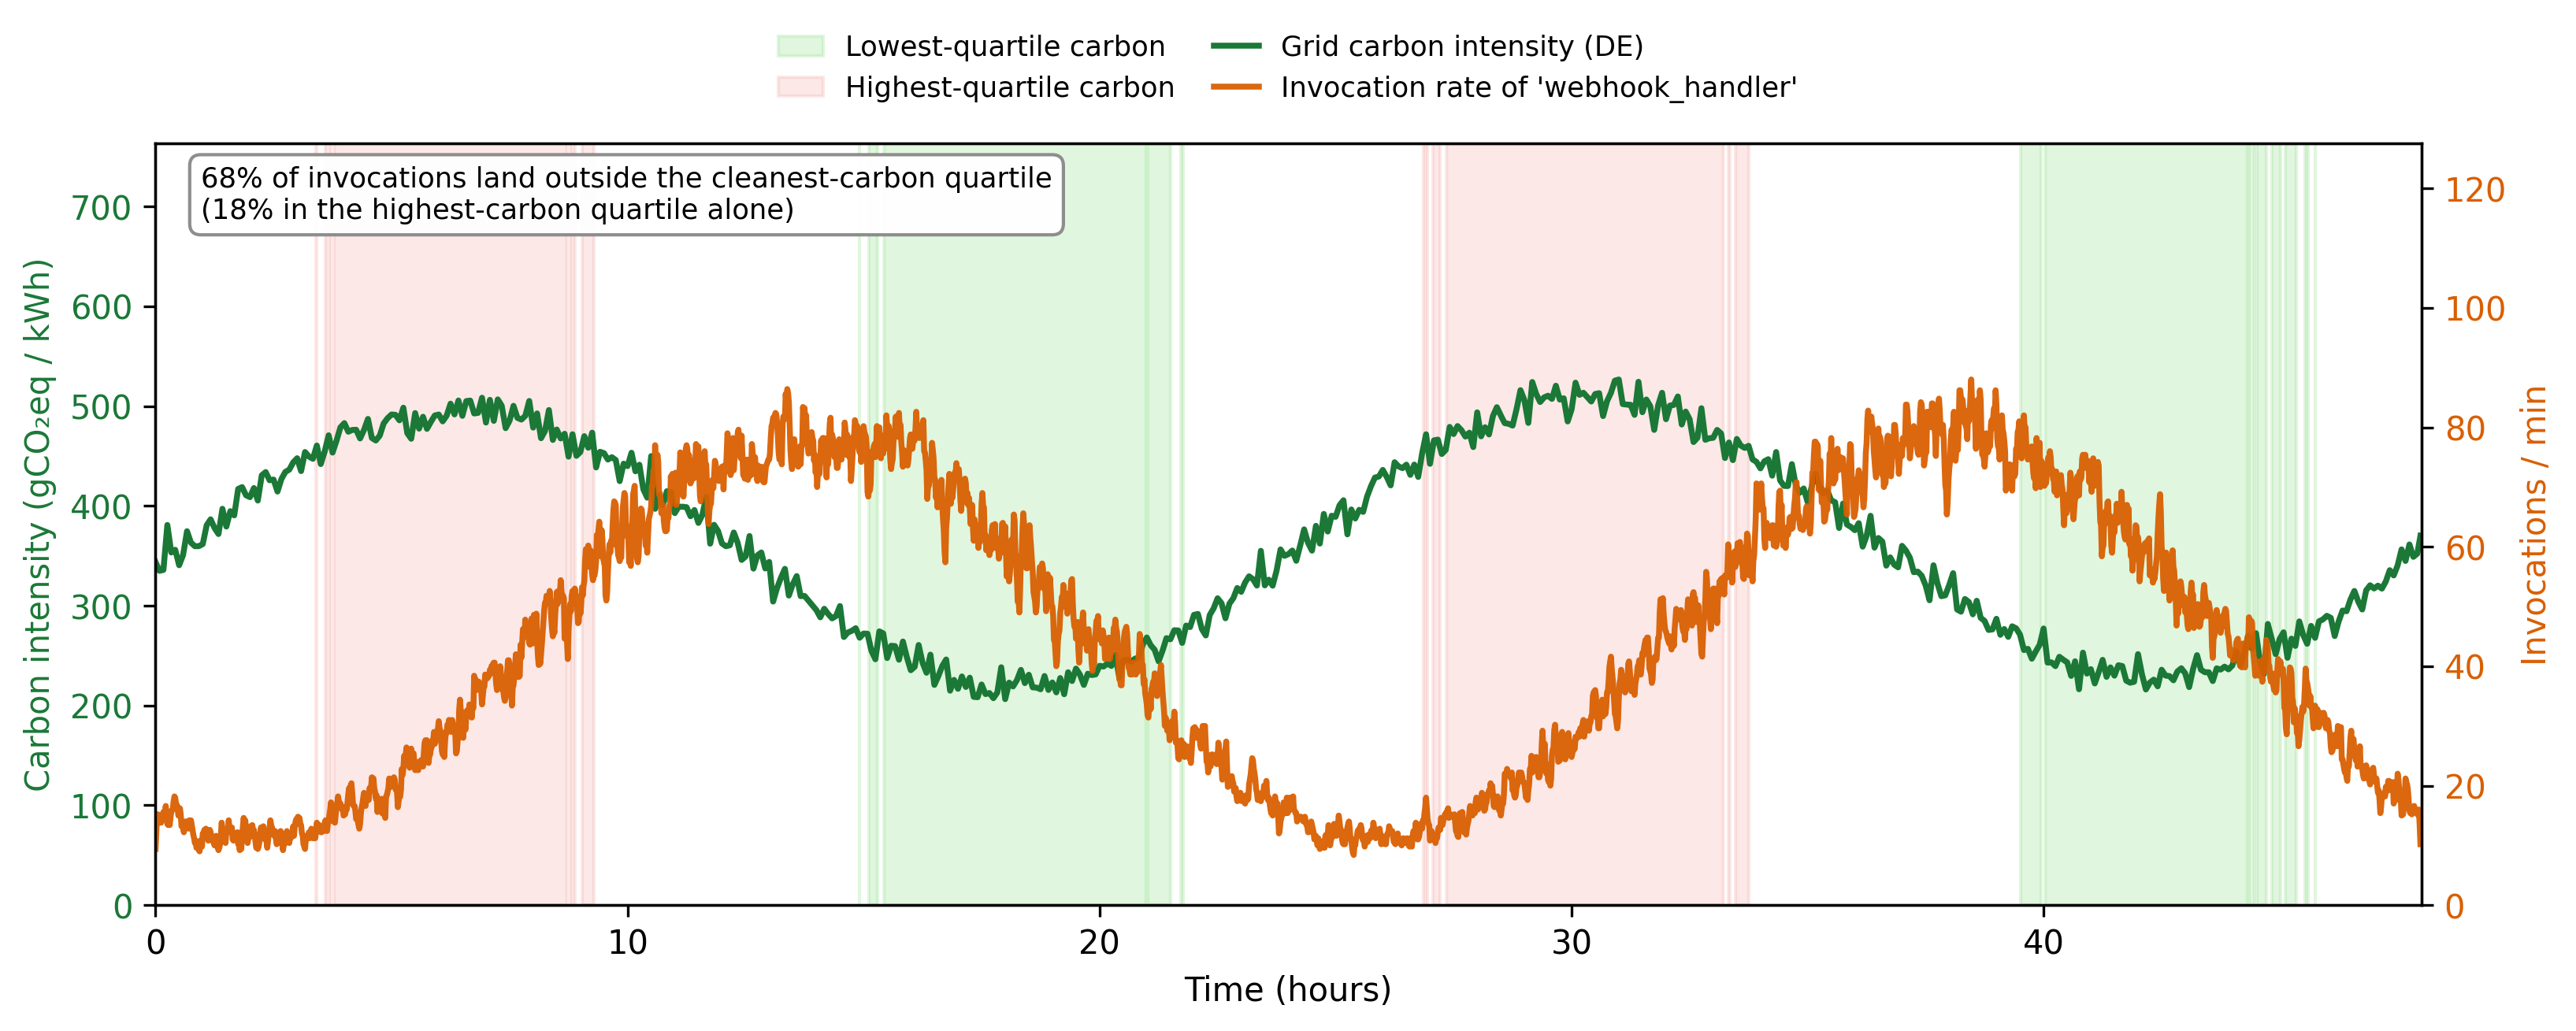
\includegraphics[width=0.95\textwidth]{figures/motivation_carbon_vs_invocations.png}
\caption{FaaS arrivals are decoupled from grid carbon intensity. The
orange line (right axis) shows the per-minute invocation rate of the
\code{webhook\_handler} function; the green line (left axis) shows
grid carbon intensity in Germany. The two signals are phase-shifted by
8--12 hours, creating temporal shifting opportunity for deferrable
invocations. Shaded bands mark the lowest- (green) and highest-carbon
(red) quartile windows.}
\label{fig:motivation}
\end{figure*}

\paragraph{1. FaaS arrival rates are decoupled from grid carbon
intensity.} The webhook function's rate follows a business-hours
diurnal pattern, peaking in early afternoon and troughing overnight.
Grid carbon intensity in Germany follows the inverse pattern: solar
and wind generation peak around midday, depressing the marginal
intensity, while night-time demand is served by base-load fossil
generation. The two signals are phase-shifted by roughly 8--12 hours;
on this representative day, 68\% of webhook invocations land
\emph{outside} the cleanest carbon quartile and 18\% land directly
in the highest-carbon quartile. The decoupling is the structural
reason carbon-aware scheduling can help.

\paragraph{2. The decoupling is robust across function classes.}
Across the 60-function catalog generated for our evaluation, the
population-weighted invocation rate correlates only weakly with the
local carbon intensity (Pearson $r$ in the range $-0.2$ to $+0.1$
across regions), confirming that arrival patterns track user activity
rather than grid economics --- as expected, since FaaS workloads are
driven by external events (user requests, message-queue depths,
scheduled triggers) that have no relationship to the regional
generation mix.

\paragraph{3. The amplitude of the carbon swing is comparable to the
amplitude of the arrival swing.} Carbon intensity in Germany swings
from $\sim$200 to $\sim$500 gCO$_2$eq/kWh over the 24-hour cycle ---
a ratio of $2.5\times$. The webhook invocation rate swings from
$\sim$15 to $\sim$80 invocations per minute --- a ratio of
$5\times$. The two signals have similar dynamic range, which means a
scheduler that can shift even a modest fraction of invocations
across the diurnal cycle has potential to capture meaningful savings.
We quantify this potential rigorously in \S\ref{sec:evaluation}.

\subsection{Implications for Scheduler Design}

The characterization directly motivates three design choices in
\S\ref{sec:algorithm}. \emph{First}, the SLA-tiered policy: arrivals
distributed across the carbon cycle are only useful to a scheduler
that distinguishes between invocations that must execute immediately
(interactive) and those that can wait. \emph{Second}, the use of
\emph{both} spatial and temporal axes: a purely temporal scheduler can
only exploit the diurnal swing within one region; a purely spatial
scheduler ignores the substantial within-region opportunity
Figure~\ref{fig:motivation} reveals. \emph{Third}, the explicit
carbon-aware warm-pool reasoning of \S\ref{sec:tradeoff}: at the
timescale of FaaS invocations (seconds), the idle-energy cost of
keeping containers warm is a first-class concern.

The motivation, in short, is not ``carbon-aware scheduling helps
FaaS'' in some generic sense --- that has been shown by the four
FaaS-targeted systems surveyed in \S\ref{sec:related:faas}
\citep{chadha2023greencourier,gsteiger2024caribou,jiang2024ecolife,qi2024casa}.
The motivation is that the \emph{specific structure} of FaaS
workloads (short, bursty, latency-tiered) combined with the
\emph{specific structure} of grid carbon traces (diurnal, decoupled
from user activity, multi-region heterogeneous) creates a joint
optimization problem that no prior scheduler has addressed in its
full generality. The rest of the paper formalizes and solves that
problem.
